Data for our preliminary results were collected using Google Forms. The
prototype would issue information to the user to take an entry survey, guide
them through the features, and finish with an exit survey. The two surveys
contained the following questions:

\begin{center}
  \begin{tabular}{|l|p{0.6\linewidth}|}
    \hline
    \multicolumn{2}{|c|}{\Large \textbf{Entry Survey}}\\
    \hline
    \multirow{6}{*}{\textbf{Demographics}}
 & Name \\ \cline{2-2}
 & Age \\\cline{2-2}
 & Gender \\\cline{2-2}
 & Education \\\cline{2-2}
 & Major \\\cline{2-2}
 & Primary OS \\
    \hline
    \multirow{6}{*}{\textbf{Usability of Shell}}
 & I think the command line is easy to use. \\ \cline{2-2}
 & I think the command line is more usable than a GUI. \\ \cline{2-2}
 & I feel comfortable using the shell. \\ \cline{2-2}
 & I prefer command line tools to GUI tools.\\ \cline{2-2}
 & I think I would prefer the shell if I understood it better (or already
   do).\\ \cline{2-2}
 & I think the shell is easy to learn.\\
    \hline
    \multirow{4}{*}{\textbf{Efficiency}}
 & I use piping and redirection. \\ \cline{2-2}
 & I use control structures in the shell.\\ \cline{2-2}
 & I use wild cards in the shell.\\
    \hline
    \multirow{5}{*}{\textbf{Knowledge}}
 & When presented with a problem, I know the commands to use. \\ \cline{2-2}
 & I feel that learning how to use new commands is easy. \\ \cline{2-2}
 & I use a wide array of commands. \\ \cline{2-2}
 & I feel that I have sufficient knowledge of the shell for what I need. \\
    \hline
    \multirow{1}{*}{\textbf{Qualitative}} & Explain what tasks you commonly carry
                                            out on in the shell.\\
    \hline
  \end{tabular}
\end{center}

\begin{center}
  \begin{tabular}{|l|p{0.6\linewidth}|}
    \hline \multicolumn{2}{|c|}{\textbf{\Large Exit Survey}} \\ \hline
    \multirow{4}{*}{\textbf{Usability}}
    & This system would improve my usage of the shell. \\ \cline{2-2}
    & This system would help me solve problems in the shell. \\ \cline{2-2}
    & This system is more usable than a traditional shell. \\ \cline{2-2}
    & I find the interface of the system inviting and usable. \\
    \hline
    \multirow{3}{*}{\textbf{Educational Value}}
    & This system would teach me commands in a more effective way than the
      status quo. \\ \cline{2-2}
    & This system would help me perform automation that I would not make on my
      own.\\ \cline{2-2}
    & Using this system would improve my understanding of all shells.\\
    \hline
    \multirow{3}{*}{\textbf{Intention}}
    & I would prefer this to the normal shell experience. \\ \cline{2-2}
    & I would use this system in the future. \\ \cline{2-2}
    & I would suggest this system to others. \\
    \hline
    \multirow{2}{*}{\textbf{Qualitative Critique}}
    & What did you like most about the system?  \\ \cline{2-2}
    & What do you think needs the most improvements? \\
    \hline
  \end{tabular}
\end{center}
In between these surveys we presented a demo of our system.

\subsection{Data Analysis}

Data analysis was carried out using the Julia and Python languages, along with
various statistical tools. A cursory data analysis was also provided by Google
Sheets, allowing an overview of the results from each question.

The first thing we wanted to do was understand the demographics of our survey.
The primary questions of age and gender did not show enough diversity to be very
statistically useful \-- almost all of the respondents were males between the
ages of 18 and 24. Education level showed a more promisingly even distribution,
and while the question of primary operating system is skewed in favor of Linux
(clearly indicating some selection bias), users of other OSes still have a
decent representation.

\begin{figure}[ht]
  \centering
  \begin{subfigure}[b]{0.45\textwidth}
\label{fig:age}
    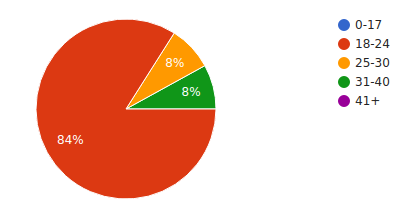
\includegraphics[width=\textwidth]{figures/stats/age.png}
    \caption{Age}
  \end{subfigure}
  \quad
  \begin{subfigure}[b]{0.45\textwidth}
\label{fig:gender}
    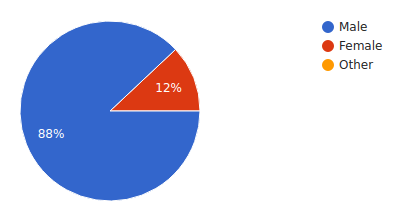
\includegraphics[width=\textwidth]{figures/stats/gender.png}
    \caption{Gender}
  \end{subfigure}

  \begin{subfigure}[b]{0.45\textwidth}
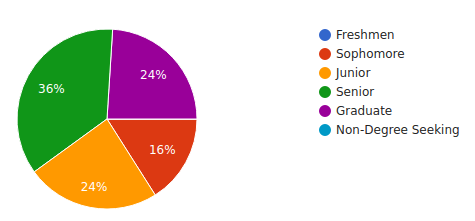
\includegraphics[width=\textwidth]{figures/stats/edu.png}
\label{fig:edu}
    \caption{Education}
  \end{subfigure}
  \quad
  \begin{subfigure}[b]{0.45\textwidth}
    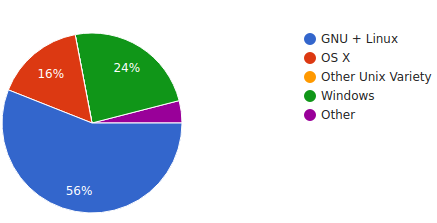
\includegraphics[width=\textwidth]{figures/stats/os.png}
\label{fig:OS}
    \caption{Primary OS}
  \end{subfigure}
  \caption{Main demographic information for survey base}
\end{figure}

Our entry survey also includes questions pertaining to the users' abilities when
using the terminal. Figure \ref{fig:skillz} shows a histogram representing a
simple additive ranking of the participants self-reported skills. The majority
of our users claim to be more experienced with the shell, which unfortunately
does not align with our target audience. However, there was still novice
representation in the data.

\begin{figure}[H]
  \centering
  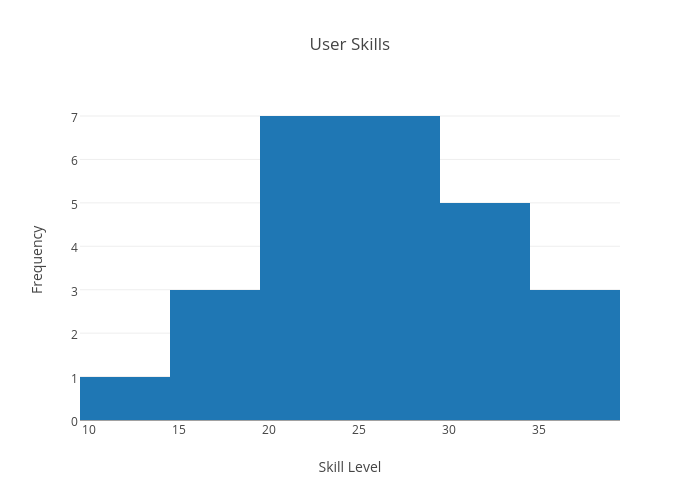
\includegraphics[width=0.6\textwidth]{figures/stats/user-skills.png}
\label{fig:skillz}
  \caption{Histogram of the relative skill levels of our users. Note the larger
    right tail.}
\end{figure}

To analyze different groups of users and their attitudes toward our prototype,
we calculated the Pearson correlation coefficient for every pair of survey
questions. To our surprise, there were no strong correlations between the
responses on the exit survey and \emph{any} of the demographic
statistics\footnote{The most significant demographic education level, which
  still had a $p$-value over $0.10$!}.  However, the data analysis did show many
interesting correlations between the questions themselves.

\begin{figure}[ht]
  \centering
  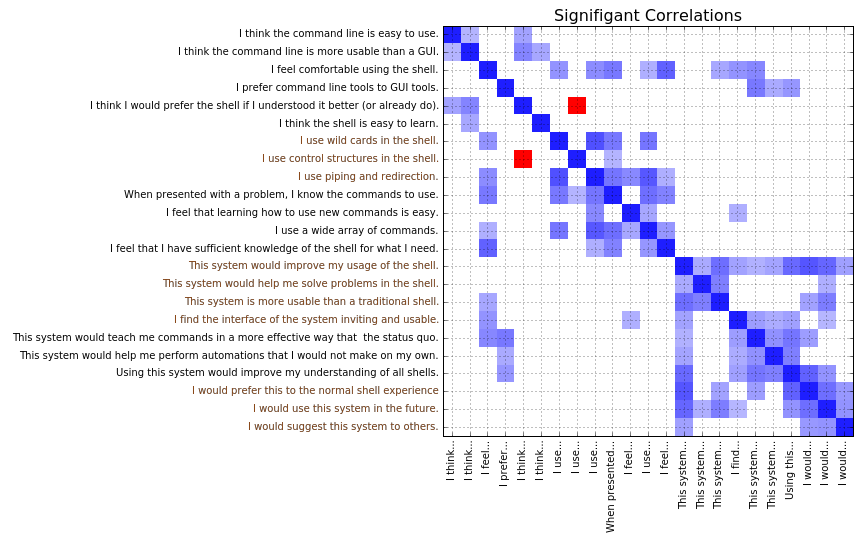
\includegraphics[width=\textwidth]{figures/stats/sig.png}
\label{fig:pvalplot}
  \caption{A matrix highlighting the Pearson correlations between each pair of
    survey questions for which the $p$-value was $< 0.05$. Darker squares
    indicate stronger correlations.}
\end{figure}

Figure \ref{fig:pvalplot} shows the statistically significant correlations between
the responses to our survey questions. A full table containing exact figures is
available in Appendix
% \ref{fig:p_table}.

Our entry survey had three groups of questions intended to serve as vectors for
a user: usability, efficiency, and knowledge. This usability vector is composed
of the questions in the top-left corner of the pearson graph. We can see that
this vector is not homogenous \-- a user's given response on one of the vector's
questions does not correlate to most of the rest of the vector's questions. The
next set, efficency, is better connected; ``I use control structures in the
shell'' is the outlier for this group. The last set on the entry survey,
knowledge, is fairly homogenous. ``I use a wide array of commands'' is correlated
with all other questions in this vector; the rest are correlated with half or
more of the vector.

Our exit survey was composed of three vectors of questions as well: usability,
education, and intention. Each of these vectors is fairly homogenous. The
usability group has a single outlier: ``I find the interface of the system
inviting and usable''. Interestingly, this question is well-correlated with the
education vector. Both the education and intention vectors are fully correlated.

The Pearson correlation matrix shows a few correlations of significance outside
of the question vectors.  From the entry survey the question most correlated to
others is ``I feel comfortable using the shell''. Users' responses to this question
have a positive correlation with two question under the efficiency vector, three
question under the knowledge vector, a single question under the usability
vector, and two questions under the education vector. This shows that users who
are more comfortable with using the shell are also more likely to self-report
being skilled users of it, unsurprisingly. From the exit survey questions, this
collection shows that users who self-reported being more comfortable with the
shell also found the prototype more usable. This might indicate that our
prototype is failing to serve our target of entry-level users.

From the exit survey the most widely associable response is a user's answer to
the question ``The system would improve my usage of the shell.'' The responses to
this question are positively correlateable to every other question on the exit
survey.

The only negative correlation of significance is between two question on the
entry survey: ``I use control structures in the shell'' and ``I think I would
prefer the shell if I understood it''.

\begin{figure}[H]
  \centering
\label{fig:alldata}
  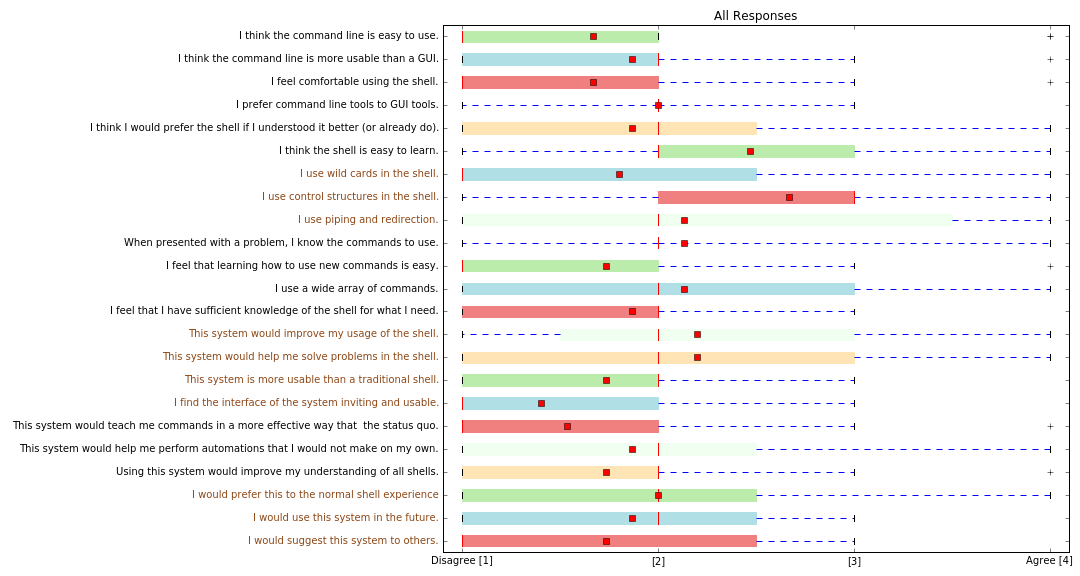
\includegraphics[width=\textwidth]{figures/stats/all.png}
  \caption{Data is free}
\end{figure}

In \ref{fig:alldata} can be seen an overview of all of our responses. There were no
correlations of significance between education levels and any response, so we
choose to analyze the data as a single group. On the entry survey most users
reported low comfort with shell usage and a preference for GUI tools. Almost all
users use piping and redirection in the shell; control structure use is less
common; most users do not use wildcards. Within the knowledge vector most users
reported difficulties with knowing and finding the information on how to
complete tasks. Most users did not feel that they used a wide array of commands.

From the exit survey we can see that most users disagreed with our prototype
being usable, educational, or a good experience.

\subsection{Qualitative Analysis}
    8d. Describe the quantitative/qualitative analysis results with proper
    statistics test/grounded theory. You should also indicate whether or not the
    analysis result can support the hypotheses in Section 8.

Our entry and exit surveys each had at least one qualitative response question.
The responses to these can be seen in Appendix
% \ref{fig:fig_data}.
The entry survey asked users what tasks they commonly carried out in the shell.
Seven out of the fifteen responses indicated navigation and file manipulation,
five indicated programming-related tasks, and four indicated searching.

There were two qualitative response questions on the exit survey. The first
asked users what they liked most about the prototype. There is no clear
consensus here \-- users reported liking the GUI elements, the context window, the
undo functionality, the suggested automations, and other disparate features.

The second asked users what they thought needed the most improvement in the
prototype. Three users indicated that more information is needed in the
interface; one wrote: ``More instructions on what the buttons on bottom will do
if pressed would be nice \-- I know the functionality of the buttons isn't
implemented yet, but a small message explaining what the buttons represent and
happens when they are clicked would go a long way.'' Two users reported
confusion with the prototype. Five did not provide an answer or indicated that
they had no suggestions.

%%% Local Variables:
%%% mode: latex
%%% TeX-master: "documentation"
%%% End:
